% Options for packages loaded elsewhere
\PassOptionsToPackage{unicode}{hyperref}
\PassOptionsToPackage{hyphens}{url}
\PassOptionsToPackage{dvipsnames,svgnames,x11names}{xcolor}
%
\documentclass[
  10pt,
]{article}
\usepackage{amsmath,amssymb}
\usepackage{iftex}
\ifPDFTeX
  \usepackage[T1]{fontenc}
  \usepackage[utf8]{inputenc}
  \usepackage{textcomp} % provide euro and other symbols
\else % if luatex or xetex
  \usepackage{unicode-math} % this also loads fontspec
  \defaultfontfeatures{Scale=MatchLowercase}
  \defaultfontfeatures[\rmfamily]{Ligatures=TeX,Scale=1}
\fi
\usepackage{lmodern}
\ifPDFTeX\else
  % xetex/luatex font selection
\fi
% Use upquote if available, for straight quotes in verbatim environments
\IfFileExists{upquote.sty}{\usepackage{upquote}}{}
\IfFileExists{microtype.sty}{% use microtype if available
  \usepackage[]{microtype}
  \UseMicrotypeSet[protrusion]{basicmath} % disable protrusion for tt fonts
}{}
\makeatletter
\@ifundefined{KOMAClassName}{% if non-KOMA class
  \IfFileExists{parskip.sty}{%
    \usepackage{parskip}
  }{% else
    \setlength{\parindent}{0pt}
    \setlength{\parskip}{6pt plus 2pt minus 1pt}}
}{% if KOMA class
  \KOMAoptions{parskip=half}}
\makeatother
\usepackage{xcolor}
\usepackage[margin=0.7in]{geometry}
\usepackage{longtable,booktabs,array}
\usepackage{calc} % for calculating minipage widths
% Correct order of tables after \paragraph or \subparagraph
\usepackage{etoolbox}
\makeatletter
\patchcmd\longtable{\par}{\if@noskipsec\mbox{}\fi\par}{}{}
\makeatother
% Allow footnotes in longtable head/foot
\IfFileExists{footnotehyper.sty}{\usepackage{footnotehyper}}{\usepackage{footnote}}
\makesavenoteenv{longtable}
\usepackage{graphicx}
\makeatletter
\def\maxwidth{\ifdim\Gin@nat@width>\linewidth\linewidth\else\Gin@nat@width\fi}
\def\maxheight{\ifdim\Gin@nat@height>\textheight\textheight\else\Gin@nat@height\fi}
\makeatother
% Scale images if necessary, so that they will not overflow the page
% margins by default, and it is still possible to overwrite the defaults
% using explicit options in \includegraphics[width, height, ...]{}
\setkeys{Gin}{width=\maxwidth,height=\maxheight,keepaspectratio}
% Set default figure placement to htbp
\makeatletter
\def\fps@figure{htbp}
\makeatother
\setlength{\emergencystretch}{3em} % prevent overfull lines
\providecommand{\tightlist}{%
  \setlength{\itemsep}{0pt}\setlength{\parskip}{0pt}}
\setcounter{secnumdepth}{-\maxdimen} % remove section numbering
\ifLuaTeX
  \usepackage{selnolig}  % disable illegal ligatures
\fi
\usepackage{bookmark}
\IfFileExists{xurl.sty}{\usepackage{xurl}}{} % add URL line breaks if available
\urlstyle{same}
\hypersetup{
  colorlinks=true,
  linkcolor={Maroon},
  filecolor={Maroon},
  citecolor={Blue},
  urlcolor={blue},
  pdfcreator={LaTeX via pandoc}}

\author{}
\date{}

\begin{document}

\section{A lossless target row with an explicit third-order parameter
factor}\label{a-lossless-target-row-with-an-explicit-third-order-parameter-factor}

2026-11-14. Source \texttt{d265c35a0efc1efb609a396e451fd543ab838c21}.
All claims unsigned {[}pcc:unverified{]}.

The actually computed norm/membership remainder has a uniform
third-order factor after evaluation at the scaled target. The identity
holds over commutative rings, including a polynomial coefficient ring in
the parameter. Its specialization is exactly the existing field model.
Replacing the constant remainder equation by the normalized target row
preserves the full five-equation solution set for nonzero parameter.
This is a concrete equation transformation for subsequent closure
analysis {[}pcc:unverified{]}.

Central claims: factor \texttt{PCC-20261114-76f2d5}, polynomial
divisibility \texttt{PCC-20261114-af9c9e}, specialization
\texttt{PCC-20261114-ca75bf}, lossless rows
\texttt{PCC-20261114-2ceac7}. \href{../lean/NormTargetFiber.lean}{Lean
source}, \href{../TARGET_FIBER_PROTOCOL.md}{contract},
\href{../target-fiber-evidence/claim-pins.json}{proof map},
\href{target-row.dot}{editable diagram}, \href{target-row.svg}{SVG},
\href{report.pdf}{PDF}.

\begin{figure}
\centering
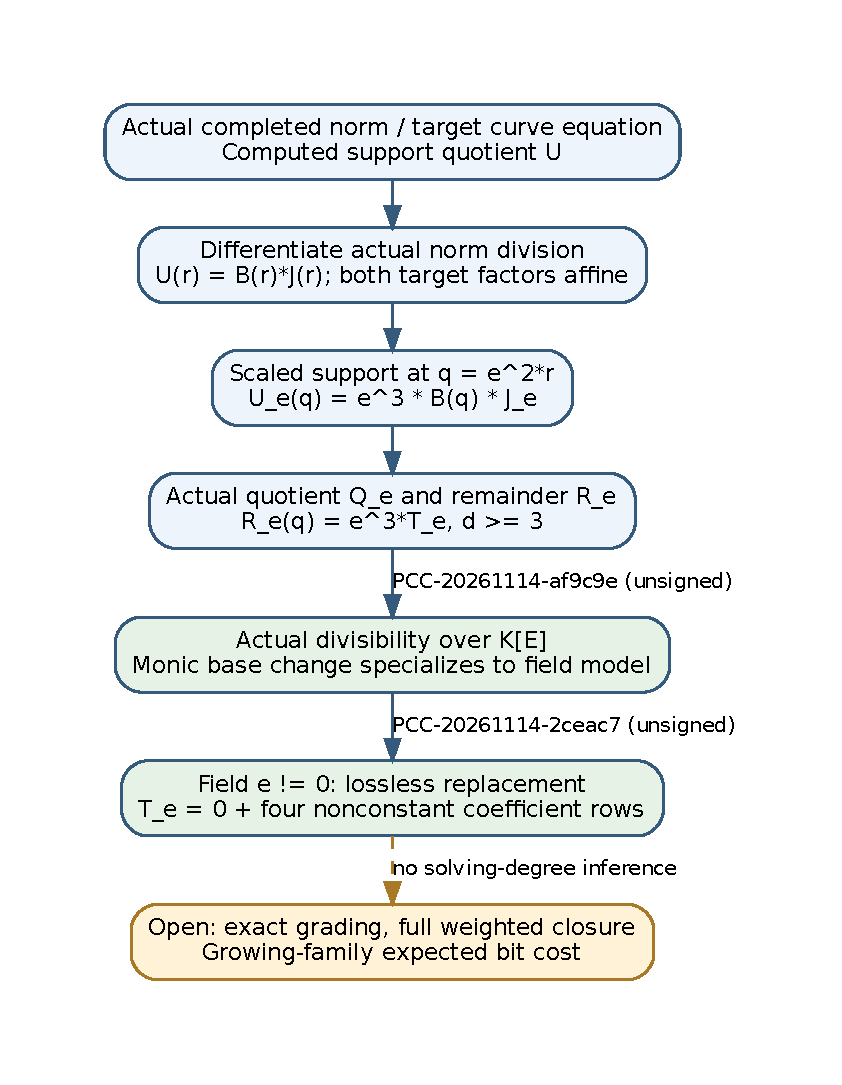
\includegraphics[width=0.9\textwidth,height=\textheight]{target-row.pdf}
\caption{The actual quotient and remainder produce the parameter factor;
specialization and nonzero-parameter row equivalence are separate
checked steps. Dashed complexity arrows remain open. Evidence unsigned.}
\end{figure}

\subsection{Construction and proof}\label{construction-and-proof}

Start with \texttt{f=X\^{}3+a*X+b}, a public target
\texttt{z\^{}2=f(r)}, \texttt{D=X\^{}3+a2*X\^{}2+a1*X}, and
\texttt{B=c0+c1*X}. Complete the actual constant:
\texttt{A=D+z*B(r)-D(r)}. The actually computed support is
\texttt{U=(A\^{}2-f*B\^{}2)\ div\ (X-r)}. Exact norm division and
differentiation give

\begin{verbatim}
U(r) = B(r)*J(r)
J(r) = 2*z*A'(r)-f'(r)*B(r)-2*z^2*B'(r).
\end{verbatim}

Differentiate the polynomial norm identity first; substitute target
values afterwards. No derivative identity
\texttt{A\textquotesingle{}=z*B\textquotesingle{}} is assumed from one
point's incidence. In this cubic/linear chart, both \texttt{B(r)} and
\texttt{J(r)} are affine expressions in the four retained coefficients.
The underlying norm derivative is established prior work; this component
builds the computed quotient and parameter-vanishing consequences on it
{[}pcc:unverified{]}.

Now use the explicit family with curve
\texttt{f\_e=X\^{}3+e\^{}4*a*X+e\^{}6*b}, target
\texttt{(q\_e,z\_e)=(e\^{}2*r,e\^{}3*z)}, and the same actual
target-completion operation. The support evaluated at that target
factors as

\begin{verbatim}
U_e(q_e) = e^3*(c0+c1*e^2*r)*J_e
J_e = 2*z*a1+4*e^2*z*r*a2+6*e^4*z*r^2
      -e*(3*r^2+a)*(c0+c1*e^2*r)-2*e^3*z^2*c1.
\end{verbatim}

For depth n put \texttt{d=2\^{}(n+1)},
\texttt{P\_e=M\_e,n-terminal*e\^{}d}, and compute
\texttt{Q\_e=P\_e\ div\ U\_e}, \texttt{R\_e=P\_e\ mod\ U\_e}. The master
recurrence gives \texttt{P\_e(q\_e)=e\^{}d*K\_n}, where
\texttt{K\_n=master(2,n)(r)-terminal} is the original public target
evaluation. Evaluating actual division yields, for d\textgreater=3,

\begin{verbatim}
R_e(q_e) = e^3*T_e
T_e = e^(d-3)*K_n-(c0+c1*e^2*r)*J_e*Q_e(q_e).
\end{verbatim}

The quotient is computed by monic division, with no free oracle or
successful coefficient witness. Norm/support degree proofs work over
nontrivial rings; actual monic remainder computation commutes with
coefficient-ring maps. Consequently this factorization is valid in
\texttt{K{[}E{]}}, with E a polynomial parameter and X the distinct
geometric variable. Mapping \texttt{E} to a field element recovers
exactly the prior \texttt{NormWeightedLeading.scaledMembership}. No
agreement-on-finite-field-values shortcut is used {[}pcc:unverified{]}.

\subsection{Exact equation replacement and
scope}\label{exact-equation-replacement-and-scope}

The actual remainder has degree below5. For any such remainder,
vanishing of its target evaluation and its four nonconstant coefficients
is equivalent to vanishing of the whole polynomial. This row replacement
is valid over the coefficient ring. Over a field, e!=0 makes e\^{}3
nonzero, so the full original five equations are equivalent to
\texttt{T\_e=0} together with those four nonconstant coefficient
equations {[}pcc:unverified{]}.

At e=1 this is an equivalent equation system for the original symbolic
input. At e=0 the polynomial divisibility remains valid, but removal of
the factor is not an asserted solution-set equivalence. The statement is
uniform divisibility by e\^{}3, not exact order3: characteristic2, z=0
or other vanishing factors can increase the order. The support/row
specialization uses this degree5 chart; no growing-arity solving theorem
is asserted {[}pcc:unverified{]}.

The expected weighted degree29 for a normalized depth4 target row
remains a graded-polynomial proof obligation. A parameter factor, input
degree or first degree fall does not establish a low weighted
last-fall/normal-form bound. Nor is a fast solver supplied by
introducing a name for the actual quotient. The original W-jet family
still needs its own faithful public map {[}pcc:unverified{]}.

\subsection{Validation, retained errors and next
test}\label{validation-retained-errors-and-next-test}

The module has26 statements. Final build007 passes; the whole-study gate
reports353 statements,0 additional trusted uses, exit0, and
import-inclusive fresh replay exits0. Standard foundations are
\texttt{propext}, \texttt{Classical.choice}, \texttt{Quot.sound}.
Validation claim \texttt{PCC-20261114-7ad52b} binds the
\href{../target-fiber-evidence/validation-001.json}{receipt}, exact
source/artifact hashes and all retained exits. All28 new source/data
claims remain unsigned; default-PATH verdicts are \texttt{not\_covered}
(exit2) {[}pcc:unverified{]}.

Dependency pins remain Lean4.35.0, CryptoLean revision
\texttt{148f5dc389b341401e06d76abe7783c4ccf42f2e}, and Mathlib revision
\texttt{cfc55fc58714a59dc06e6e79edc6d1d95140d3c2}. The adapter uses
Rust1.99.1. No earlier mathematical source, dependency, checker/hash or
gate changed {[}pcc:unverified{]}.

Literal certificate \texttt{IDC1h085fdef17210ed0e}, claim
\texttt{PCC-20261114-365b89}, seals only the unconditional evaluated
derivative-factor step

\begin{verbatim}
2*Z*B*D-F*B^2-2*Z^2*B*C = B*(2*Z*D-F*B-2*Z^2*C).
\end{verbatim}

Its syntactic degree is4, with32 statement-derived and16 extra replay
points. It does not encode the curve premise, parameter divisibility,
specialization, row equivalence or execution. The canonical adapter's22
tests, format, release build and issuance pass; strict clippy records
four inherited style failures in unchanged canonical SHA256. Failed
proof drafts002/004/006 retain export-body equality, mapped numeral and
wrong factor-side errors. Drafts001/003/005 and final007 pass. No check
was suppressed {[}pcc:unverified{]}.

No native fixture/closure experiment, unknown-root search, F4/msolve,
paid/cloud/attack run or timing comparison was attempted. The earlier
fixed fixture flow remains1 planned,0 attempted,0 completed,0 excluded,1
admission- blocked by unchanged checkpoint upload transport. Pure Lean
and literal certificate construction are separate. The old sparse
benchrec1680/162 diagnostic is preserved; this change touches no
benchmark records or progress/gate generator {[}pcc:unverified{]}.

Sources checked (KB): unavailable as already recorded; no unchanged
retry. The
\href{../target-fiber-evidence/prior-search-receipt.json}{bounded
fallback} records five queries and exact URLs. Read actual NormWronskian
derivative, public-jet rigidity and functional/polarization sources;
earlier theory and rationality reviews preserve scheme/field-selection
limits. Their Kummer- coset rationality lemma is not transferred to the
Dickson input. Reuse the primary weighted-GB and ML full-closure
reviews; neither input degree nor first-fall behavior supplies a solver
bound. No novelty or exhaustive- absence claim follows from this
token-matching search {[}pcc:unverified{]}.

Next, prove the graded interpretation of the normalized target row and
construct a bounded full-closure/normal-form certificate. Any
computational test needs its own unchanged acceptance criteria and
checkpoint admission; one successful cell would not prove growing-family
scaling. The broad goal still requires an efficient public-input finder
and complete expected bit cost, including field extraction, useful
relations and verification {[}pcc:unverified{]}.

Global performance/curve/attack-route graphs remain unchanged: there is
no new measured speed or group-transport edge. Earlier
source/evidence/claims and canonical ledger bytes remain intact. This
study's new diagram separates the exact algebraic transformation from
the open complexity arrow {[}pcc:unverified{]}.

\subsection{Exact proof map}\label{exact-proof-map}

Exact hypotheses and declaration hashes are in claim-pins.json. All
entries are unsigned {[}pcc:unverified{]}.

\begin{longtable}[]{@{}ll@{}}
\toprule\noalign{}
NormTargetFiber declaration & Unsigned claim \\
\midrule\noalign{}
\endhead
\bottomrule\noalign{}
\endlastfoot
\texttt{normDerivativeRing} & \texttt{PCC-20261114-075987} \\
\texttt{linearQuotientValue} & \texttt{PCC-20261114-9bf216} \\
\texttt{normQuotientTargetFactor} & \texttt{PCC-20261114-25d287} \\
\texttt{supportTargetValue} & \texttt{PCC-20261114-20bbfa} \\
\texttt{remainderTargetIdentity} & \texttt{PCC-20261114-e5137c} \\
\texttt{scaledCurveEquation} & \texttt{PCC-20261114-e0d47c} \\
\texttt{scaledSupportTargetValue} & \texttt{PCC-20261114-1cd56e} \\
\texttt{masterAtScaledTarget} & \texttt{PCC-20261114-8d052a} \\
\texttt{membershipTargetFactor} & \texttt{PCC-20261114-76f2d5} \\
\texttt{membershipTargetDivisibility} & \texttt{PCC-20261114-7a2d78} \\
\texttt{polynomialParameterDivisibility} &
\texttt{PCC-20261114-af9c9e} \\
\texttt{normWindowRing} & \texttt{PCC-20261114-cef811} \\
\texttt{supportWindowRing} & \texttt{PCC-20261114-5fb4da} \\
\texttt{scaledSupportWindowRing} & \texttt{PCC-20261114-4a71b9} \\
\texttt{targetRowsIff} & \texttt{PCC-20261114-5a50b9} \\
\texttt{membershipTargetRowsIff} & \texttt{PCC-20261114-18d3c7} \\
\texttt{mapActualA} & \texttt{PCC-20261114-d9cee2} \\
\texttt{mapSupport} & \texttt{PCC-20261114-ac74c3} \\
\texttt{mapMaster} & \texttt{PCC-20261114-3b0238} \\
\texttt{mapMembership} & \texttt{PCC-20261114-58ed53} \\
\texttt{scaledSupportField} & \texttt{PCC-20261114-76fbe7} \\
\texttt{masterField} & \texttt{PCC-20261114-f20511} \\
\texttt{membershipField} & \texttt{PCC-20261114-6be927} \\
\texttt{parameterSpecialization} & \texttt{PCC-20261114-ca75bf} \\
\texttt{normalizedTargetEquation} & \texttt{PCC-20261114-6f0e15} \\
\texttt{membershipNormalizedRowsIff} & \texttt{PCC-20261114-2ceac7} \\
\end{longtable}

\end{document}
